\documentclass[12p]{article}
\setlength{\parindent}{0em}
\usepackage{amsmath, mathrsfs, listings}
\usepackage{upquote, amssymb}
\usepackage[utf8]{inputenc}
\usepackage[english]{babel}
\usepackage[%
    left=0.50in,%
    right=0.50in,%
    top=1.0in,%
    bottom=1.0in%
]{geometry}%
\usepackage{graphicx}
\graphicspath{ {./images/} }
\renewcommand{\baselinestretch}{1.5}

\begin{document}

\section{(1) Adjon formulat abszolut folytonos eloszlasu X valoszínusegi valtozo eseten az Y = g(X) valoszínusegi valtozo varhato ertekere!}

\section{(2) Legyen X standard normalis eloszlasu valoszínusegi valtozo. Szamítsa ki az X varhato erteket! }

\section{(3) Mondja ki Bayes tetelet. (3x)}

Legyen B1, B2, ..., pozitív valoszínusegu esemenyekbol allo teljes esemenyrendszer, A $\in$ $\mathscr{A}$ pozitív valoszínusegu. Ekkor

$$\displaystyle{P(B_k|A) = \frac{P(A|B_k)P(B_k)}{\displaystyle{\sum_i} P(A|B_i)P(B_i)}}$$

\section{(4) Igazolja, hogy fuggetlen azonos parameteru binomialis eloszlasu valoszínusegi valtozok osszege is ilyen.}

\section{(5) Írja fel az X es Y egyuttes eloszlasfuggvenye es az X perem eloszlasfuggvenye kozott fennallo kapcsolatot.}

\section{(6)  Definialja a szorasnegyzetet es mondja ki legfontosabb tulajdonsagait. (3x)}

$$D^2X = E[(X - E(X))^2] = EX^2 - E^2X$$

Tulajdonsagok:

\begin{itemize}
	\item $D^2(X) \geq 0$, mert nemnegatív valoszínosegi valtozo varhato erteke
	\item $D^2(aX+b)=a^2D^2(X)$, mert $D^2(aX+b)=E[(aX+b-E(aX+b))^2]= E[(aX+b-aE(X)-b)^2]=E[(aX-aE(X))^2]=a^2 E[(X-E(X))^2]$.
	\item Abbol, hogy $E(X)$ veges, meg nem kovetkezik $D^2(X)$ vegessege, hiszen ha $P(X=k)=c/k^3$ (egyertelmoen megadhato olyan c, amire ez eloszlas lesz) akkor $E(X)$ veges, de $E(X^2)=c(1+1/2+...+1/k...)$, ami vegtelen.
\end{itemize}

\section{(7) Definialja a konfidencia-intervallum fogalmat (3x)}

A konfidenciaintervallum a valoszínusegi intervallum, az induktív statisztika eszkoze: ha mintabol becsulunk, sosem tudjuk a pontos erteket, a teljes sokasag felmerese igen draga dolog. A konfidenciaintervallum adott szignifikanciaszinten: a becsult valtozo also es felso korlatja.

(8) -

\section{(9) Adja meg a linearis regresszio feladatat es megoldasat.}

Az $Y = a_1X_1 + a_2X_2 + · · · + a_pX_p + b$ egyenletben az
egyutthatok es a konstans meghatarozasa

Azaz:

$$\min_{a_1, ..., a_p,b} g(a_1,...,a_p,b) = \min_{a_1,...,a_p,b} E(Y - (a_1X_1 + ... + a_pX_p+b))^2$$

Megoldasa:

b szerinti derivalt:

$$\frac{\partial g}{\partial b} = -2E(Y - (a_1X_1 + ... + a_pX_p + b)) = 0$$

Kifejezve b-t:

$$b = EY - a_1EX_1 - ... - a_pEX_p$$

$a_i$ (i = 1, . . . , p) szerinti derivalt:

$$\frac{\partial g}{\partial a_i} = -2E((Y-(a_1X_1 + ... + a_pX_p + b))X_i) = 0$$

b-t behelyettesítve az $a_i$ szerinti derivaltba:

\begin{align*}
0  &= -2E((Y - (a_1X_1 + ... + a_pX_p + b))X_i)\\
 &= -2E\left(\left((Y - EY) - \sum_{j = 1}^p a_j(X_j - EX_j)\right)X_i\right)\\
 &= -2(E(YX_i) - EYEX_i) +\\
 &+ 2 \sum_{j=1}^p a_j(E(X_iX_j) - EX_iEX_j)\\
 &= -2Cov(Y,X_i) + 2\sum_{j=1}^p a_j Cov(X_i,X_j), \quad i=1,...,p
\end{align*}

Jeloles: $C := Var(\underline{X})$, $d := Cov(Y, \underline{X})$
Ebbol a kovetkezo egyenletrendszert kapjuk:
$$C\underline{a} = \underline{d}$$
melynek egyertelmu megoldasa, ha C regularis:
$$\underline{a} = C^{-1}\underline{d}$$
A masodik derivalt vizsgalataval belathato, hogy ez
valoban minimum

\section{(10) Definialja idosorok eros stacionaritasat.}

Eros stacionaritas: az egyuttes eloszlasok nem
fuggnek az idotol

\section{(11) Definialja az ASN fogalmat.}

Az eljaras hatekonysagat mero szam: varhato mintaelemszam

$ASN = n_1 = n_2(1 - P^{I}_a - P^I_r)$, ahol $P_a^I$ annak valoszínusege, hogy az elso minta alapjan atvegyuk a tetelt, a $P_r^I$ pedig a visszautasítas valoszínusege.

\section{(12) írja fel az eloszas- es a surusegfuggvenyeket karakterizalo tulajdonsagokat! (3x)}

Eloszlasfuggveny:\\
$F_X(z):=P(X<z)$. $F_X(z):\mathbb{R}\rightarrow\mathbb{R}$ fuggveny az X valoszínusegi valtozo eloszlasfuggvenye.\\
Tulajdonsagai:

\begin{itemize}
	\item $0 \leq F_X(z) \leq 1$
	\item $F_X(z)$ monoton no
	\item $\lim_{z \rightarrow \infty} F_X(z) = 1; \lim_{z \rightarrow -\infty} F_X(z) = 0$
	\item $F_X(z)$ balrol folytonos
\end{itemize}

Surusegfuggveny:\\
Az X valoszínusegi valtozo surusegfuggvenye $f(x) \leftrightarrow X$-re:

$F_X(z) = \int_{-\infty}^z f(t) dt$

Tulajdonsagai:
\begin{itemize}
	\item $f \geq 0$
	\item $\int_{-\infty}^{\infty} f(t) dt = 1$
	\item Minden ilyen f integralfuggvenye eloszlasfuggveny
\end{itemize}

\section{(13) Legyen X pascal eloszlasu valoszínusegi valtozo. Szamítsa ki az X varhato erteket!}

$$EX = \frac{1}{p}$$

\section{(14) Mi a kapcsolat az X es Y valoszínusegi valtozo fuggetlensege es egyuttes eloszlasfuggvenye kozott? (3x)}

Fuggetlen esetben az egyuttes eloszlasfuggveny a peremeloszlasfuggvenyek szorzatabol kaphato meg.

\section{(15) írja fel, az X diszkret valoszínusegi valtozo varhato ertekenek definíciojat! (2x)}

Egy X diszkret valoszínusegi valtozo (aminek az ertekkeszlete
$R_X$ es $i \in R_X$ eseten $P(X = i) = p_i)$ $E(X)$ varhato erteke a lehetseges ertekeinek a valoszínusegekkel sulyozott atlaga, ha ez a sor abszolut konvergens.

$$E(X) = \sum_{i \in R_X} i * p_i$$

Ha a sor nem abszolut konvergens, akkor azt mondjuk, hogy nem letezik a varhato ertek.

(16) -

\section{(17) Vezesse le a polinomialis eloszlas koordinatai kozotti korrelaciora vonatkozo kepletet.}

\section{(18) Definialja a Poisson folyamatot. (3x)}

Poisson folyamat: idoben lejatszodo folyamatnal adott [a,b) intervallumba eso esemenyek szama $(X_{a,b})$ eppen $\lambda(b-a)$ parametero Poisson eloszlasu, ha a folyamat

\begin{itemize}
	\item homogen: $X_{a,a+t}$ eloszlasa csak t-tıl fugg;
	\item utohatas nelkuli: $X_{a,b}$ es $X_{b,c}$ fuggetlenek ha a<b<c;
	\item nemelfajulo: $0<P (X_{a,b}=0)<1$.

\end{itemize}

\section{(19) Mondja ki a nagy szamok torvenyenek minel tobb valtozatat. (3x)}

	\subsection{Gyenge torveny}
	
	$X_1, X_2, ...$ fuggetlenek, azonos eloszlasuak, $EX_i = m < \infty$, $D^{2}X_i = \sigma^2 < \infty$. \\
	$P(\frac{X_1 + ... + X_n}{n} - m \geq \varepsilon) \rightarrow 0$ $(n \to \infty)$ $\forall \varepsilon > 0$-ra (sztochasztikus konvergencia).
	
	\subsection{Eros torveny}
	
	$X_1, X_2, ...$ fuggetlenek, azonos eloszlasuak, $EX_1 = m < \infty$, $D^{2}X_1 = \sigma^2 < \infty$. \\
	$\frac{X_1 + ... + X_n}{n} \rightarrow m$ $(n \to \infty)$ 1 valoszínuseggel. \\
	Megjegyzes: Csebisev-egyenlotlenseggel bizonyítjuk. ($\frac{\sigma^2}{n \varepsilon^2} \to 0$ $(n \to \infty)$)
	
	\subsubsection{Csebisev-egyenlotlenseg}
	
	$EX$ veges. \\
	Ekkor $P(|X-EX| \geq \lambda) \leq \frac{D^{2}X}{\lambda^2}$ \\
	Megjegyzes: Bizonyítas Markov-egyenlotlenseggel.
	
	\subsubsection{Markov-egyenlotlenseg}
	
	$X \geq 0, c > 0$. \\
	Ekkor $P(X \geq c) \leq \frac{EX}{c}$
	


\section{(20) Vezesse le a Poisson eloszlas parameterere a maximum likelihood becslest. (3x)}

Zyxon megoldasas:

A likelihood fuggveny:

$$L(\theta;\underline{x}) = f_{\theta}(\underline{x}) = \prod^n_{i=1} f_{\theta}(x_i)$$

Ennek maximumhelye lesz a $\theta$ parameter maximum likelihood becslese. A Poisson-eloszlas parametere: $\overline{X}$

Tankonyvar.hu-s megoldas:

$$P(X_1 = k) = \frac{\lambda^k}{k!}e^{-\lambda}\quad k=0, 1, 2, ...$$
A likelihood-fuggveny
$$L(x_1, ..., x_n;\lambda)=\prod^n_{i=1}\frac{\lambda^{x_i}}{x_i!}e^{-\lambda}$$
A loglikelihood-fuggveny
$$l(x_1, ..., x_n;\lambda) = \sum^n_{i=1}(x_i log \lambda - \lambda - log x_i!)$$
A maximumhelyet derivalassal hatarozzuk meg:
$$0 = \frac{\theta l(x_1, ..., x_n;\lambda)}{\theta \lambda} = \frac{1}{\lambda} \sum^n_{i=1} x_i - n$$
Innen
$$\hat{\lambda} = \frac{1}{n} \sum^n_{i=1} X_i = \overline{X}$$
A maximum-likelihood becsles.

\section{(21) Definialja a linearis modell hipoteziseit es adja meg a probastatisztikat.}

$H_0: a = 0$ tesztelese t-probaval:

$$t_{n-2} = \frac{\hat{a} \sqrt{(n-2) \sum_{i=1}^n(x_i - \overline{x})^2}}{\sqrt{\sum_{i=1}^n (y_i - \hat{a}x_i- \hat{b})^2}}$$

$H_0:b=0$ tesztelese t-probaval:

$$t_{n-2} = \frac{\hat{b} \sqrt{n(n-2)\sum_{i=1}^n (x_i - \overline{x})^2}}{\sqrt{\sum_{i=1}^n (y_i - \hat{a}x_i - b)^2}\sqrt{\sum_{i=1}^n x_i^2}}$$

\section{(22) Legyen X +1 es -1 erteket felvevo valoszínusegi valtozo, $P(X = 1) = 1/6$ es $P(X = -1) = 5/6$. Szamítsuk ki X varhato erteket es szoras negyzetet.}

$$ E(X) = \frac{1}{6} * 1 + \frac{5}{6} * -1 = 2/3$$

$$ EX^2 = 1^2 * \frac{1}{6} + (-1)^2 * \frac{5}{6} = 1$$

$$ D^2(X) = EX^2 - E^2X = 1 - \left(\frac{2}{3}\right)^2 = \frac{5}{9}$$

\section{(23) Bizonyítsa be a nagy szamok gyenge torvenyet. (2x)}

\section{(24) Legyen $X^2$ egyenletes a $[0, 1]$-en. Adja meg X eloszlasat es varhato erteket.}

\section{(25) Irja fel a rendezett minta k-adik elemenek a surusegfuggvenyet.}

\section{(26) Rajzolja fel, hogyan lehet a surusegfuggvenyek segítsegevel a probak kritikus ertekeit es erofuggvenyuket szemleltetni!}

\section{(27) Definialja a $\chi$-negyzet probat es adja meg legfontosabb alkalmazasait.}

A Pearson-fele khí-negyzet ($\chi^2$) proba diszkret eloszlasu vagy ilyenne teheto valtozok vizsgalatara alkalmas statisztikai eljaras.

Illeszkedesvizsgalat $\displaystyle{\sum_{i=1}^r \frac{(v_i - np_i)^2}{np_i}}$\\
Homogenitasvizsgalat: $\displaystyle{nm \sum_{i=1}^r \frac{(\frac{v_i}{n}-\frac{\mu_i}{m})^2}{v_i + \mu_i}}$\\
Fuggetlensegvizsgalat: $\displaystyle{T_n = \sum_{i=1}^r \sum_{j=1}^s 
\frac{(v_{ij} - \frac{v_{i\cdot}v_{\cdot j}}{n})^2
}{\frac{v_{i\cdot}v_{\cdot j}}{n}}}$

\section{(28) Adja meg a linearis regresszio feladatat es alkalmazasait.}

A statisztika eszkoztaraban a linearis regresszio egy olyan parameteres regresszios modell, mely feltetelezi a magyarazo- (X) es a magyarazott (y) valtozo kozti (parametereiben) linearis kapcsolatot. Ez azt jelenti, hogy linearis regresszio becslese soran a mintaveteli adatok pontfelhojere igyekszunk egyenest illeszteni.

Hasznalhato pl.:

\begin{itemize}
	\item Termekek arai es a vasarlasi szamok osszefuggese
	\item eletkor es a halalozas kapcsolata
	\item Koltseg tullepesi valtozok
\end{itemize}

\section{(29) Vezesse le a normalis eloszlas varhato ertekere a momentum modszerrel adodo becslest.}

\section{(30) Adjon modszert idosorok simítasara.}

Idosor simítasa: kiszuri a rovidtavu ingadozasok hatasat,
eltunteti a szezonalitast

\begin{itemize}
	\item Mozgoatlag modszer
	\item Exponencialis simítas
\end{itemize}

(31) -

\section{(32) Mondja ki a centralis hatareloszlas tetelt. (2x)}

151.-es kerdesben benne van a valasz.

\section{(33) Legyen $X$ olyan valoszínusegi valtozo, amely a (0, 1) intervallumbol veszi fel az ertekeit. Eloszlasfuggvenye ott F(t) = t/2 ha $t \in (0, 1/2]$, es $F(t) = 3/4 + t/4$ ha $t \in (1/2, 1]$. Rajzoljuk fel X eloszlasfuggvenyet es szamítsuk ki a $P(X \leq 1/2)$, valamint a $P(1/4 \leq X \leq 3/4)$ es $P(X = 1/2)$ valoszínusegeket!}

\section{(34) Definialja a teljes esemenyrendszer fogalmat! (2x)}

Esemenyek $A_1, A_2, ...,$ sorozata teljes esemenyrendszer, ha
egymast paronkent kizarjak es egyesítesuk $\Omega$.

\section{(35) Definialja a folytonos eloszlasokra a varhato ertek fogalmat.}

$$EX = \int_{-\infty}^{\infty} x f(x) dx$$
ha az integral letezik.

\section{(36) Mondja ki Bernstein tetelet.}

Legyen $(X_1, X_2, ..., X_n)$ olyan, hogy $D^2(X_1) + D^2(X_2) ... + D^2(X_n) < kn$, valamint tegyuk fel, hogy van olyan $h: N \rightarrow R_{+}$ fuggveny, melyre $|R(X_i, X_j)| \leq h(|i-j|)$ es $\frac{1}{n} \displaystyle{\sum^n_{i=1}} h(i) \rightarrow 0$ ekkor $(X_1 + ... + X_n) / n - (m_1 + m_2 + ... + m_n)/n \rightarrow 0$ sztohasztikusan.

\section{(37) Bizonyítsa be a Markov egyenlotlenseg altalanos alakjat.}

77.-es kerdesben!

\section{(38) Definialja a maximum-likelihood modszert.}

Azt a parametererteket keressuk, ahol a likelihood fuggveny a legnagyobb erteket veszi fel (azaz diszkret esetben az
ismeretlen parameter azon erteket keressuk, amely mellett a bekovetkezett eredmeny maximalis valoszínusegu): $\max_{\theta}L(\theta; x)$.

Ez nyilvan megegyezik azzal a parameterertekkel, ahol a log-likelihood fuggveny veszi fel a legnagyobb
erteket, azaz: $\max_{\theta} l(\theta; x)$.

Amennyiben a fuggveny derivalhato $\theta$ szerint, akkor a maximumot kereshetjuk a szokasos modon, a derivaltak
segítsegevel, azonban a feladatunkat jelentosen megnehezíti, hogy olyan n-szeres szorzatot kellene derivalni, amelyiknek minden tagjaban ott van az a valtozo, ami szerint derivalnunk kellene. Ezert likelihood fuggveny helyett a log-likelihood fuggveny maximumhelyet keressuk.

Ha $\theta$ 1 dimenzios, akkor $\partial_\theta l(\theta, x) = 0$, míg ha $\theta = (\theta_1, ..., \theta_p)$ p dimenzios, akkor $\partial_{\theta_i} l(\theta, x) = 0$ megoldasabol
kapjuk a becslest. (A masodik derivaltak segítsegevel ellen ˝orizz¨uk, hogy valoban maximum.)


\section{(39) Definialja a Wilcoxon probalt.}

Ez a proba olyan kíserleti helyzetekben alkalmazhato, ahol a mintavetel a paros megfigyelesen alapul, ahol 2 osszefuggo valtozobol mintavetel tortenik, ugy, hogy mindegyikbol egy-egy jut egy megfigyelesi egysegbe.

A proba feltetelei:
\begin{itemize}
	\item Ordinalis skalan merheto folytonos valoszínusegi valtozok eseten akkor alkalmazhato,
	\item ha a kulonbsegek is ordinalis skalan merhetoek.
	\item Erosen asszimmetrikus eloszlas eseten nem alkalmazhato.
\end{itemize}

\section{(40) Definialja az autoregresszios es a mozgoatlag folyamatokat.}

Autoregresszív folyamat

Az $Y_t$ diszkret parameteru sztochasztikus
folyamatok k-ad rendu autoregresszív
folyamatnak nevezzuk, ha

$$Y_t = \alpha_1 * Y_{t-1} + \cdots + \alpha_k * Y_{t-k} + \mathcal{E}_t$$

Ahol:\\
$\alpha_i$ konstansok\\
$Y_t$ feher zaj (varhato erteke 0, szorasa $\sigma_y$)

Mozgoatlag-folyamat

Az $Y_t$ diszkret parameteru sztochasztikus
folyamatot k-ad rendu mozgoatlag folyamatnak
nevezzuk, ha

$$Y_t = \beta_0 * U_t + \beta_1 * U_{t-1} + \cdots + \beta_k * U_{t-k}$$

Ahol\\
$\beta_k$ konstansok\\
$U_t$ diszkret feher zaj (varhato ertek 0, szoras $\sigma_u$)

\section{(41) Mit jelent a becsleses illeszkedesvizsgalat es hogyan alkalmazzuk ra a $\chi$-negyzet probat?}

Legyen $\theta$ egy $s$ dimenzios parametervektor, valamint legyen $\hat{\theta}$ a $\theta$ parametervektor ML-becslese, es legyen $\hat{p}_j = p_j(\hat{\theta})$

$H_0 : P(X_i = x_j) = \hat{p}_j \quad j=1,\cdots,r$\\
$H_1 : \exists$ legalabb egy j melyre $P(X_i = x_j) \neq \hat{p}_j$\\
Probastatisztika: $$T_n = \sum^r_{j=1} \frac{(v_j - n\hat{p})_j)^2}{n\hat{p}_j} \stackrel{H_0 eseten}{\sim} \chi^2_{r-s-1}$$
Kritikus tartomany: $$\chi_k = \{x: T_n(x) > \chi^2_{r-s-1,1-\alpha}\}$$

\section{(42) Legyen X n-edrendu p parameteru binomialis eloszlasu valoszínusegi valtozo. Szamítsa ki az X varhato erteket!}

$$EX = np$$

\section{(43) Mondja ki a szita (Poincare) formulat.}

Keplet az altalanos esetre:

$$P(A_1 \cup A_2 \cup ... \cup A_n) = \sum^n_{i=1} (-1)^{i+1} S^{(n)}_i$$
ahol
$$S^{(n)}_i = \sum_{1 \leq j_1 < j_2 < ... < j_i \leq n} P(A_{j_1}, \cap A_{j_2} \cap ... \cap A_{j_i})$$

az i tenyezıs metszetek
valoszínosegeinek osszege.

\section{(44) Definialja a kovarianciat es írja le tulajdonsagait. (4x)}

$cov(X,Y) := E[(X-E(X))(Y-E(Y))]$

Kiszamítasa:
$cov(X,Y) = E(XY)-E(X)E(Y)$

Ha X es Y fuggetlenek $\rightarrow$ $cov(X,Y) = 0$, fordítva nem feltetlenul igaz

A kovariancia szimmetrikus: $cov(X,Y) = cov(Y,X)$

$cov(X,X) = D^2(X)$

\section{(45) Mondja ki a centralis hatareloszlas tetel lokalis valtozatat. (2x)}

Legyenek $X_1 , X_2 ,..., X_n ,...$ fuggetlen, azonos eloszlasu, abszolut folytonos valoszínosegi valtozok. Tegyuk fel, hogy $\sigma_2=D_2(X)$ veges $(m:=E(Xi))$ es hogy $f(x)$ korlatos. Tekintsuk a standardizalt osszeguket:

$$Z_n := \frac{X_1 + ... + X_n - nm}{\sqrt{n}\sigma}$$

Ekkor $Z_n$ surusegfuggvenye konvergal a standard normalis
eloszlas sorosegfuggvenyehez, azaz

$$\lim_{n \rightarrow \infty} f_n(x) = \frac{1}{\sqrt{2\pi}} e^{- \frac{x^2}{2}}$$

A konvergencia z-ben egyenletes.

\section{(46) Legyen X egyenletes a [0,1]-en. Adja meg $X^2$ eloszlasat es varhato erteket.}

\section{(47) Irja fel a Nadarajah modszer lenyeget es szemleltesse grafikusan az eljaras motivaciojat! }

Ha csak mert adataink vannak, kozelítjuk a
felteteles varhato erteket (hasonlo a ParzenRosenblatt becsleshez).

$$\hat{r}_n(x) = \frac{\displaystyle{\sum^n_{i=1} Y_ik \left(\frac{x - X_i}{h_n}\right)}}{\displaystyle{\sum^n_{i=1} k \left(\frac{x - X_i}{h_n}\right)}}$$

A Parzen-Rosenblatt tetel feltetelei eseten ez
konzisztens becslese az E(Y|X) regresszionak.

\section{(48) Definialja a 2 mintas t-probat es vezesse le a probastatisztika kepletet!}

\textit{t-proba}:	Ennel a probanal nem ismert a szoras, viszont ugyanugy normalis eloszlast feltetelezunk, mint az u-probanal. $\xi_i \sim N(m, \sigma^2)$, $i=1..n$.

\textit{Ketmintas}: $\xi_i \sim N(m_1, \sigma_1^2)$, $i=1..n$ es $\eta_j \sim N(m_2, \sigma_2^2)$, $j=1..m$. Ez esetben sem ismert a szoras, viszont feltetelezzuk, hogy a ket minta szorasa megegyezik. Ekkor 
$$\displaystyle{t = \sqrt{\frac{nm}{n+m}}\frac{\overline{X} - \overline{Y}}{\sqrt{\frac{(n-1)(s^*_1)^2 + (m-1)(s^*_2)^2}{n+m-2}}} \stackrel{H_0 eseten}{\sim}
t_{n+m-2}}$$
$n+m-2$ a proba szabadsagfoka.

\section{(49) Mondja ki a Neyman-Pearson lemmat!}

A proba legerısebb a sajat terjedelmevel. Minden legerısebb proba ilyen alaku

\section{(50) Definialja az autokorrelacios egyutthatokat es adja meg becslesuket arra az esetre, amikor rezidualisokbol szamolunk!}

\section{(51) Definialja a valoszínusegi mezo fogalmat! (2x)}

($\Omega, \mathcal{A}, P$) Kolmogorov-fele
valoszínusegi mezo, ha
\begin{itemize}
	\item $\Omega$ nemures halmaz
	\item $\mathcal{A}$ az $\Omega$ reszhalmazainak $\sigma$-algebraja
	\item $P: \mathcal{A} \rightarrow [0, 1]$  halmazfuggveny
(valoszínuseg) , melyre
	\item $P(\Omega) = 1$
	\item $\sigma$-additivitas: ha $A_1, A_2,\cdots,$ paronkent
kizaro esemenyek, akkor $P(A_1 \cup A_2 \cup \cdots) = P(A_1) + P(A_2) + \cdots$
\end{itemize}

\section{(52) Vezesse le, hogy a korrigalt tapasztalati szorasnegyzet torzítatlan becsles a szorasnegyzetre. }

\section{(53) Vezesse le, hogy a relatív gyakorisag konzisztens becsles a valoszínusegre.}

\section{(54) Definialja becslesek aszimptotikus torzítatlansagat.}

$T_n(X)$ a $\theta$ parameter konzisztens becslese, ha
$$E_{\theta}(T_n(\underline{X})) \rightarrow \theta$$

\section{(55) Definialja a t-probat az egy- es ketmintas esetre is.}


Egymintas
$\sigma$ ismeretlen; Probastatisztika:

$$T(X) = t = \frac{\overline{X} - m_0}{\frac{s^{*}_n}{\sqrt{n}}} \stackrel{H_0 eseten}{\sim} t_{n-1}$$

Kritikus tartomanyok:

$$\chi_k = \{X: |t| > t_{n-1,1-\alpha/2}\} \quad \chi_k = \{X: t > t_{n-1,1-\alpha}\} \quad \chi_k = \{X: t < t_{n-1, \alpha}\}$$

Ketmintas

Probastatisztika:

$$\displaystyle{t = \sqrt{\frac{nm}{n+m}}\frac{\overline{X} - \overline{Y}}{\sqrt{\frac{(n-1)(s^*_1)^2 + (m-1)(s^*_2)^2}{n+m-2}}} \stackrel{H_0 eseten}{\sim}
t_{n+m-2}}$$

\section{(56) Definialja a szekvencialis probat (egyszeru hipotezisek esetere).}

A valoszínoseghanyados n elemo mintabol

$$\displaystyle{V_n = \frac{\prod^n_{i=1} f_1(X_i)}{\prod^n_{i=1} f_0(X_i)}}$$

\begin{itemize}
\item Addig veszunk mintaelemeket, amíg $V_n \geq B$ vagy $V_n \leq A$ nem teljesul\\
Tehat az algoritmus:
\item $V_n \geq B$: elutasítjuk $H_0$-t
\item $V_n \leq A$ : elfogadjuk $H_0$-t.
\item $B>Vn>A$: uj mintaelemet veszunk.
\end{itemize}

\section{(57) Definialja a korrelacios egyutthatot es mondja ki legfontosabb tulajdonsagait.}

A valtozok kozotti linearis kapcsolat erosseget mero
mennyiseg a korrelacios egyutthato: 

$$R(X, Y) = \frac{cov(X,Y)}{D(X)D(Y)}$$

Tulajdonsagai:

\begin{itemize}
\item $R(X,Y)=0$, ha X es Y fuggetlenek (ez sem
fordíthato meg)
\item Ez alapjan definício szerint legyen R(X,Y)=0, ha X
vagy Y elfajult eloszlasu.
\item $R(X,aX+b)=1$, ha $a>0$, mert $cov(X,aX+b)=aD^2(X)$
\end{itemize}


\section{(58) Mikor nevezunk egy torzítatlan becslest hatasosabbnak egy masiknal?}

$T_1$ hatasosabb becslese a $\theta$ parameternek a $T_2$-nel, ha
$$D_{\theta}^2(T_1(\underline{X})) \leq D_{\theta}^2(T_2(\underline{X}))$$
teljesul minden $\theta$ parameterertekre.

\section{(59) Definialja idosorokra a trend es a periodus fogalmat.}

Kulonbozo, eltero tartalmu
komponensekre bontott idosor, additív vagy multiplikatív
formaban felepítve. Pl.: additív esetben

$$Y_t = T_t + C_t + S_t + u_t$$

ahol T, C es S a trend, a ciklikus es a periodikus komponens,
u pedig a veletlen folyamat.

\section{(60) Adjon peldat olyan maximum likelihood becslesre, ami nem torzítatlan! (3x)}

$$\gamma^2 = \frac{\sum(X_i - \overline{X})^2}{(n-1)}$$

\section{(62) Definialja valoszínusegi valtozok eloszlasat.}

Mivel a gyakorlati problemaknal $\Omega$ nem
mindig adhato meg egyertelmuen, es
absztrakt halmazok helyett szívesebben
dolgozunk a valos szamokkal, a kulcsfogalom
a valoszínusegi valtozok eloszlasa.\\
Legyen B tetszoleges Borel halmaz.
$Q_X(B):= P{\omega: X(\omega) \in B}$ valoszínuseget ad
meg R Borel halmazain. Ez az X eloszlasa.\\

\section{(63) Mit jelent a valoszínuseg folytonossaga?}

Ha $A_i \in \mathcal{A} (i = 1,2,\cdots)$ es $A_1 \supseteqq A_2 \supseteqq \cdots$ akkor az $\displaystyle{A = \cap^{\infty}_{i=1}A_i}$ jelolessel $\lim_{n \rightarrow \infty} P(A_n)=P(A)$

\section{(64) Definialja n valoszínusegi valtozo fuggetlenseget.}

 Az $X_1,...,X_n$ valoszínusegi valtozok fuggetlenek, ha az $\mathscr{F}_{X1}, \mathscr{F}_{X2} ,...,\mathscr{F}_{X_n}$ generalt $\sigma$-algebrak fuggetlenek.

\section{(65) Definialja diszkret valoszínusegi valtozok egyuttes eloszlasat!}

az X diszkret valoszínusegi valtozo, ha ertekkeszlete $(x_1 ,..., x_n...)$ legfeljebb megszamlalhato.\\
A valoszínusegi valtozo definíciojabol adodoan $\{\omega:X(\omega)= x_i\}=\{X=x_i\}= \in \mathscr{A}$ azaz $p_i:=P$ $(X=x_i)$ertelmes. Ezek meg is hatarozzak X eloszlasat.

\section{(66) Definialja a t eloszlast!}

Definício:  Az X  valoszínusegi valtozot $n$ szabadsagfoku Student eloszlasunak nevezzuk, ha surusegfuggvenye:

$$f(x) = \frac{\Gamma \left(\frac{n+1}{2}\right)}{\sqrt{\pi} \sqrt{n \Gamma} \left(\frac{n}{2}\right) \left(1 + \frac{x^2}{n}\right)^{\frac{n+1}{2}}}$$

\section{(67) Definialja a gyenge konvergenciat!}

$P_n \rightarrow P$ gyengen, ha minden $f: S \rightarrow R$ folytonos, korlatos fuggvenyre

$$\int fdP_n \rightarrow \int fdP$$

Tulajdonsagok: tobbek kozott azzal is
ekvivalens, hogy $P_n(A) \rightarrow P(A)$ minden P-folytonossagi halmazra.

\section{(68) Irja fel annak a valoszínuseget, hogy a 90/5-os lottonal egy szelvennyel jatszva legalabb 2 talalatunk lesz!}

\section{(69) Legyen az alabbi 3 megfigyelesunk az $(X, Y)$ parra. $(1;2)$ $(1.2;2.5)$ $(0.8;1.6)$. Nadarajah
modszeret hasznalva a $k(x) = 1$, ha $-1/2 < x < 1/2$ (es 0 kulonben) magfuggvennyel es a $h = 0.5$ ablakszelessegel, mi lesz az $E(Y|X = 1.1)$ becslese?}

\section{(70) Vezesse le egyszeru hipotezisekre, hogy az egymintas u-proba valoszínuseghanyadosproba az egyoldali ellenhipotezis eseten!}

\section{(71) Hogyan tudjuk a linearis modellt alkalmazni polinommal torteno kozelítesre?}

\section{(72) Adjon peldat olyan maximum likelihood becslesre, mely nem torzítatlan.}

\section{(73) Definialja az elojelprobat! Mik a kritikus ertekek? (3x)}

Nemparameteres proba, illeszkedesvizsgalat $\rightarrow$ adott eloszlasu-e a minta?

Az elojelproba a kulonbsegek elojelen alapul. $H_0$ eseten Binom(n; 1/2).

\section{(74) Adjon peldat olyan $X_n$ valoszínusegi valtozo-sorozatra, amely fuggetlen tagu, de megsem teljesul ra a centralis hatareloszlastetel.}

\section{(75) Legyen X egyenletes eloszlasu a [-1, 1] intervallumon. Szamítsa ki $X^2$ surusegfuggvenyet.}

\section{(76) Definialja a normalis eloszlast es vezesse le a legfontosabb tulajdonsagait.}

Feltuno tulajdonsaga a normalis eloszlasnak, hogy nem ferde, illetve az atlagra szimmetrikus. Ez azt jelenti, hogy a normalis eloszlas atlaga, medianja es modusza egyenlo. A normalis eloszlas alakjat haranghoz szokas hasonlítani.

$N(m, \sigma^2)$; Eloszlasfuggveny: visszavezetheto $\Phi$-re\\ Surusegfuggveny: $$\displaystyle{\frac{1}{\sqrt{2\pi} \sigma}e^{-\frac{(x-m)^2}{2\sigma^2}}}$$

EX: m\\
$D^2X: \sigma^2$

\section{(77) Mondja ki es bizonyítsa is be a Markov egyenlotlegnseget.}

Legyen $g : \mathbb{R} \rightarrow \mathbb{R}$ monoton novo pozitív fuggveny, $X \geq 0$ valoszínusegi valtozo, melyre $EX < \infty$ es $\mathcal{E} > 0$ tetszoleges. Ekkor

$$P(X \geq \mathcal{E}) \leq \frac{E(g(X))}{g(\mathcal{E})}$$

Spec., ha $g(x) = x$, akkor

$$P(X \geq \mathcal{E}) \leq \frac{EX}{\mathcal{E}}$$

Bizonyitas diszkret esetre

$$E(X) = \sum_{i \in R_X} i*p_i = \sum_{i>0,i\in R_X} i*p_i \geq \sum_{i \geq a, i\in R_X} i*p_i \geq \sum_{i\geq a, i\in R_X} a*p_i = aP(X \geq a)$$

Bizonyitas folytonos esetre

$$E(X) = \int_{-\infty}^{\infty} yf_X(y)dy = \int_{0}^{\infty} yf_X(y)dy \geq \int_{a}^{\infty} yf_X(y)dy$$
$$\int_{a}^{\infty}yf_X(y)dy \geq \int_{a}^{\infty} af_X(y)dy = a * P(X \geq a)$$

\section{(78) Hogyan alkalmazhatjuk a Kolmogorov-Szmirnov probat veletlenszam-generatorok tesztelesere?}

A tapasztalati es az elmeleti eloszlasfuggveny
legnagyobb eltereseit karakterizalja

$$K_n^{+} = \sqrt{n} \max (F_n(x) - F(x)), \quad K_n^{-}=\sqrt{n} \max(F(x) - F_n(x))$$

Tablazatbol kiolvashato a keresett valoszínuseg\\
A kis lokalis eltereseket nem mutatja ki

\section{(79) Definialja a binomialis eloszlast, vezesse le a kepletet es adja meg alkalmazasi lehetosegeit!}

\subsection{Levezetes}

Amennyiben N ugy tart a vegtelenhez, hogy kozben $M/N \rightarrow p$ (ahol $p \in (0,1)$), akkor a hipergeometrikus eloszlas tart a binomialis eloszlashoz:

$$\lim_{N \rightarrow \infty, N/M \rightarrow p} {M \choose k}{{N - M} \choose {n - k}}/{N \choose n} = {n \choose k}p^k(1-p)^{n-k}$$

\subsection{Alkalmazas}
\begin{itemize}
\item Visszateveses mintavetel mas realizacioja: fuggetlen kíserletek azonos korulmenyek kozott. $P(A) = p$ esemeny, vegezzunk n(rogzített szamu) fuggetlen kíserletet.
\item X: az A bekovetkezesenek gyakorisaga (pontosan hanyszor jott ki az A). X eloszlasa binomialis (n,p).
\item $X = X_1 + X_2 + \cdots + X_n$ ahol $X_i$ az i-edik kíserletnel az A esemeny indikatora. Ezek az indikatorok fuggetlenek is!

\end{itemize}

\section{(80) Legyenek az adataink: 1,2,5,6. Szamolja ki a mediant es rajzolja fel a tapasztalati eloszlasfuggvenyt!}

\section{(81) Tegyuk fel, hogy egy 10 fos csoportban mindenki kihuzza valakinek a nevet a karacsonyi ajandekozasnal. varhato ertekben hany ember huzta sajat magat? Vezesse is le az eredmenyt!}

\section{(82) Rajzolja fel a $\lambda = 1$ es $\lambda = 2$ parameteru exponencialis eloszlas suruseg- es eloszlasfuggvenyet!}

\section{(83) Vezesse le a $[0, \theta]$ intervallumon egyenletes eloszlasra a maximum likelihood becslest n mintaelem alapjan!}

\section{(84) Rajzolja fel az alabbi minta tapasztalati eloszlasfuggvenyet: 1,5,6,7! (2x)}

\section{(85) Hogyan tudunk inverz modszerrel veletlen szamot generalni? (2x)}

Legyen X val. valt., F eloszlasfuggvennyel,
amely monoton novekedı es folytonos. Ekkor

\begin{itemize}
	\item F(X) egyenetes eloszlasu [0, 1]-en.
	\item Ha $U \sim U(0, 1)$ akkor $F^{-1}(U)$ eloszlasfuggvenye F.
\end{itemize}

Pl.:

$$X \sim exp(\lambda) \rightarrow F(x) = 1-exp(-\lambda x) \rightarrow F^{-1}(x) = -\ln (1-x)/\lambda \rightarrow -\ln(1-U)/\lambda \sim exp(\lambda)$$

\section{(86) Legyen az X valoszínusegi valtozo surusegfuggvenye $f(x) = x^2/9$, ha $0 < x < 3$ es $0$ kulonben. Adjuk meg $X$ eloszlasfuggvenyenek erteket az $1/2$ helyen. $E(1/X)=?$ Adjuk meg $sqrt{X}$ surusegfuggvenyenek erteket az $1/2$ helyen.}

\section{(87) Szamítsa ki annak a valoszínuseget, hogy egy haromgyerekes csaladban azonos nemuek a gyerekek! (Tegyuk fel, hogy a fiuk es lanyok szoletesi valoszínusege is 0.5 es hogy az egyes szuletesek fuggetlenek.)}

\section{(88) Definialja a varhato ertek fogalmat diszkret valoszínusegi valtozokra!}

A $p_i =P (X=x_i)$ eloszlassal megadott valoszínosegi valtozo varhato erteke $E(X):= p_1x_1+ p_2x_2 +...,$ ha a sor abszolut konvergens.

\section{(89)  Legyen X egyenletes eloszlasu a $[-2,2]$ intervallumon. Adja meg $(X - 2)(X + 2)$ surusegfuggvenyet.}

\section{(90) Mondja ki abszolut folytonos valoszínusegi valtozok fuggetlensegenek ekvivalens jellemzoit. (2x)}

Ha X koordinatai fuggetlenek, akkor definício szerint:

$F_X(z) = P(X_1<z_1, X_2<z_2, ..., X_d<z_d) = F_1(z_1)F_2(z_2)...F_n(z_n) \forall z \in \mathbb{R}^d$

\section{(91) Mondjon peldat az egyenletes, az exponencialis es a normalis eloszlas alkalmazasara!}

Egyenletes eloszlas:\\
Veletlengeneratorokban igyekeznek az egyenletes eloszlast egy adott intervallumon minel inkabb kozelíteni

Exponencialis eloszlas:\\
Elorejelzeseknel alkalmazzak: n adatpontos minta megfigyelese utan egy ismeretlen exponencialis eloszlasu forrasbol meg tudjuk josolni, hogy mi lesz a kovetkezo ertek ugyanabbol az ismeretlen exponencialis eloszlasu adatforrasbol

Normalis eloszlas:\\
Meresi hibakra, mert ingadozasokra es olyan elettartam vizsgalatokra hasznaljuk, ahol a keszulekek, alkatreszek rendszeres kopassal mennek tonkre. Bizonyos feltetelek esetek a binomialis eloszlas kozelítesere is hasznalhato.

\section{(92) Definialja a bootstrap modszert.}

\begin{itemize}
	\item Adott $X_n$-bol m elemu visszateveses mintat veszunk (altalaban m=n) \quad $X^{*}_m = \{X^{*}_1,...,X^{*}_m\}$
	\item $X_i^{*}$ kozos eloszlasa: $F_n = n^{-1} \sum^n_{i=1} \delta_{x_i}$
	\item $T^{*}_{m,n} = t_m (X^{*}_m;F_n)$
	\item Ismetles $\rightarrow \hat{G}_{m,n}$
	
\end{itemize}


\section{(93) Mi a leíro statisztika feladata?}

Celja egy mar rendelkezesre allo, valosagra vonatkozo adathalmaz osszefoglalasa, elemzese, egyszoval az informaciotomorítes.\\

\section{(94) Definialja a kovarianciat!}

$$cov(X, Y) = E(XY) - EXEY$$

\section{(95) Mihez tart $P(X1+X2+ ... +Xn > 9n/2)$, ha $X1, X2, . . .$ fuggetlen, a $[4,6]$ intervallumon
egyenletes eloszlasu valoszínusegi valtozok es n tart vegtelenhez?}

\section{(96) Vezesse le az exponencialis eloszlas varhato ertekere vonatkozo kepletet!}

$$E \xi = \int^{\infty}_0 x \cdot \lambda \cdot e^{-\lambda x} dx = [-x \cdot e^{-\lambda x}]^{\infty}_0 + \int^{\infty}_0 e^{-\lambda x} dx = \left[\frac{e^{-\lambda x}}{-\lambda} \right]^{\infty}_0 = \frac{1}{\lambda}$$

\section{(97) Legyen az alabbi 3 megfigyelesunk az $(X, Y)$ parra. $(1;2)$ $(1.3;2.5)$ $(0.8;1.5)$. Nadarajah
modszeret hasznalva a a $k(x) = 1$, ha $-1/2 < x < 1/2$ (es 0 kulonben) magfuggvennyel es a $h = 0.5$ ablakszelesseggel, adjon becslest $Y$ kozelítesere, ha $X = 1$.}

\section{(99) Az alabbi minta: 0,0,1,1,2 alapjan becsuljuk torzítatlanul az alabbi parametereket:
varhato ertek, szorasnegyzet, annak a valoszínusege, hogy $X > 0.2$.}

\section{(100) Adjon modszert arra, hogyan szimulalna veletlen szamot a $\sin x (0 < x < \pi/2)$ surusegfuggvenyu eloszlasbol!}

\section{(101) Hogy hívjuk a $h(t) = E(|X - t|^2)$ fuggveny minimum helyet?}

\section{(102) Hogyan adhatjuk meg a megszamlalhato valoszínusegi mezon a valoszínuseget?}

$$P(A) = P(\cup_{i:\omega_i \in A} \omega_i) = \sum_{i:\omega_i \in A} p_i$$

\section{(103) Legyen X 5 varhato erteku es 2 szorasu normalis eloszlasu, Y pedig az X = 7 esemeny indikatora. Szamítsa ki Y varhato erteket es szorasat!}

\section{(104)  Definialja a visszateves nelkuli mintavetel modelljet es adja meg a kulonbozo selejtszamok valoszínusegeit!}

N termek, melybol M selejtes\\
n elemo minta visszateves nelkul\\
A: pontosan k selejtes van a mintaban
(k=0,...,n)

$$P(A) = \frac{{M \choose k}{{N - M} \choose {n - k}}}{{N \choose n}}$$

\section{(105) Mondja ki a Markov egyenlotlenseget!}

77.-es kerdesben!

\section{(106) Vezesse le a valoszínusegre a maximum likelihood becslest n mintaelem alapjan!}

\section{(107) Definialja a sztochasztikus konvergenciat! (2x)}

 minden $\mathcal{E}$, $\delta>0$-
hoz megadhato olyan $n_0$, hogy $n>n_0$ eseten $P(|X_n-X| \geq \mathcal{E}) \leq \delta$.

Lemma

$$X_n \rightarrow X m.m. \leftrightarrow \lim_{m \rightarrow \infty} P(\sup_{n \geq m} |X_n - X| > \mathcal{E}) = 0$$

Kov.: A m.m. konvergenciabol kovetkezik a
sztochasztikus konvergencia.


\section{(108) Írja le a surusegfuggveny becslesere tanult eljarast.}

$$f_n(x) = \frac{1}{nh_n}\sum^n_{i=1}k\left( \frac{x-X_i}{h_n} \right)$$

\section{(109) Adja meg a legkisebb negyzetes becslest a linearis modellben. Mik a tulajdonsagai?}

\section{(110) Legyen X egyenletes a $[0, 1]$-en. Adja meg $X^2$ eloszlasat es varhato erteket.}

\section{(111) Szamolja ki a Wilcoxon probastatisztika erteket az alabbi ket adatsorra! Hogyan dontene arrol, hogy tekinthetok-e azonos eloszlasbol szarmazonak? Az elso minta: 1,2,4,12,23,50;
a masodik minta: 3,8,15,25,61,200.}

\section{(112) Definialja az F-probat es adja meg legfontosabb alkalmazasait. (2x)}

$$H_0: \sigma_1 = \sigma_2$$
$$H_1: \sigma_1 \neq \sigma_2$$
Probastatisztika
$$F= \frac{(s_1^{*})^2}{(s_2^{*})^2} \stackrel{H_0 eseten}{\sim} F_{n-1,m-1}$$

\section{(113)  Hogyan generalhatunk veletlen szamot Neumann modszerevel?}

Legyen f(x) tetszoleges surusegfuggveny, $g(x)$ pedig olyan surusegfuggveny, amelyre $f(x) < Mg(x)$, valamely $M>1$ eseten es $g(x)$-bol konnyen tudunk mintat venni (tipikus pelda az egyenletes eloszlas).

\section{(114) Toltse ki az alabbi tablazat hianyzo cellait ugy, hogy a peremeloszlasok egyenletesek
legyenek a megadott szamokon! Fuggetlenek-e ezek a valtozok? Szamolja ki az $E(X^2Y)$ varhato erteket!}

\begin{center}
 \begin{tabular}{| c c || c | c | c | c |} 
 \hline
 Y & X &  0 & 1 & 2 & 3\\ [0.5ex] 
 \hline\hline
 0 &  & 0,2 & & 0,05 & \\ 
 \hline
 1 &  & & 0,15 & & \\
 \hline\hline
\end{tabular}
\end{center}

\section{(115) Mutassa meg, hogy fuggetlen azonos parameteru binomialisok osszege binomialis eloszlasu! Mi a kapcsolat a rendek kozott?}

\section{(116) Definialja ket esemeny fuggetlenseget!}

Az A es B esemenyek fuggetlenek, ha $P(A \cap B) = P(A)P(B)$.

\section{(117) Szamítsa ki ket kockadobas maximumanak a varhato erteket.}

\section{(118) Definialja az elso- es masodfaju hiba fogalmat, valamint probak konzisztenciajat.}

Elso:\\
Valamely nullhipotezis statisztikai probaval vegzett vizsgalataban az a hiba, amelyet a nullhipotezis elutasítasa jelent amikor az igaz. Valoszínûsege az elsõfaju kockazat (alfa). 

Masodfaju hiba\\
Az a hibas dontes, hogy nem vetjuk el a helytelen nullhipotezist abban az esetben, amikor az alternatív hipotezis igaz. A proba kozvetlenul nem ellenõrzi, ezert ha a proba nem utasítja el a nullhipotezist, ez meg nem jelenti azt, hogy a nullhipotezist megfelelõ statisztikai biztonsaggal elfogadhatjuk. Valoszínûsege a masodfaju kockazat (beta). 

Konzisztencia\\
Az erofv. 1-hez tart (minden $\theta \in \Theta_1-re$)


\section{(119) Irja le a t-proba alkalmazasat a parosított megfigyelesek esetere.}

Pelda: Van-e kulonbseg Budapest es Cegled napi atlaghımerseklete kozott?$H_0: m_1=m_2$ a nullhipotezis. 

Ha ugyanazon napokrol van megfigyelesunk
mindket helyen: nem fuggetlenek a mintak.
Ekkor a parok tagjai kozotti kulonbseget
vizsgalva, az elozo egymintas esetre
vezethetı vissza a feladat. $H_0*: m=0 ,H_1^{*}:m\neq0$ az uj hipotezisek. 


\section{(120) Vajon van-e stacionarius megoldasa az $X_n = 0.96 X_{n-1} + \epsilon_n$ rekurzionak? Valaszat
indokolja!}

\section{(121) Legyen a mintaelemek surusegfuggvenye $f(x) = (\theta + 1)x^{\theta}$ ha $0 < x < 1$ ($\theta \geq$ 0 a par.).
Egy mintaelem alapjan hatarozzuk meg az $\alpha = 0.05$ terjedelmu valoszínuseghanyadosprobat a $H_0 : \theta = 0, H_1 : \theta = 1$ hipotezisekre!}

\section{(122) Ismertesse a linearis regresszio egyutthatoira vonatkozo probak lenyeget! (2x)}

??

\section{(123) Adott n elemu minta az alabbi eloszlasbol: $P(Z = 1) = c$, $P(Z = 2) = 2c$, $P(Z = 3) = 1 - 3c$ ($0 < c < 1/3$ az ismeretlen parameter). Hatarozza meg a parameter maximum likelihood becsleset!}

\section{(124) Szamítsa ki ket kockadobas minimumanak a varhato erteket.}

\section{(125) Írja fel a Csebisev egyenlotlenseget, es vazolja a bizonyítasat.}

Legyen X tetszoleges valoszínusegi valtozo, melyre $D^2X < \infty$ es $\mathcal{E} > 0$ tetszoleges. Ekkor

$$P(|X - EX| \geq \mathcal{E}) \leq \frac{D^X}{\mathcal{E}^2}$$

Bizonyítas:

Az $Y = |X - E(X)|$ valoszínusegi valtozora írjuk fel a Markov-egyenlotlenseg erosebb formajat.

$$g(a)P(|X - E(X)| \geq \mathcal{E}) \leq E(g(|X - E(X)|))$$

Ekkor ha a $g(x) = x^2$, ha $x > 0$, egyebkent 0 fuggvenyt írjuk be (ami monoton novo):

$$\mathcal{E}^2P(|X - E(X)| \geq \mathcal{E}) \leq E((|X - E(X)|)^2) = E((X - E(X))^2) = D^2(X)$$

\section{(126) Legyen X 5 varhato erteku Poisson eloszlasu, Y pedig az X = 5 esemeny indikatora. Szamítsa ki Y varhato erteket es szorasat!}

\section{(127) Adjon peldat olyan maximum likelihood becslesre, mely nem torzítatlan.}

pl. a normalis eloszlas szorasnegyzetere kapott becsles ilyen

\section{(128) Adja meg a Wilcoxon-proba hipoteziseit, a probastatisztikat es a kritikus tartomanyt.
Mikor alkalmazna ezt a probat? (2x)}

???

\section{(129) Adjon meg ket modszert integralok szimulacioval torteno kiszamítasara! Hasonlítsa is
ossze oket!}

\begin{itemize}
\item Integralok kozelítese
\item Bootstrap
\end{itemize}

Az elso eljaras is torzítatlan es szorasnegyzete $(E(g^2(X)) - I^2) / N$, amibol kisebb szoras adodik.\\
Tovabb is javíthato, ha X az [a,b]-ra koncentralodo f surusegfuggvenyu eloszlasbol szarmazik:
$$\int^b_a g(x)dx = \int^a_b \frac{g(x)}{f(x)} f(x)dx = E (\frac{g(X)}{f(X)})$$
es ennek meg kisebb a szorasa, ha $f(X) \approx g(X)$\\
Tehat g(X)/f(X) szimulalt ertekeinek atlaga jo kozelítes\\
Az is elonye, hogy improprius integralokra is alkalmazhato (ha pl. f a normalis eloszlas)

\section{(132) Vezesse le a normalis eloszlas varhato ertekere a maximum likelihood becslest n mintaelem alapjan!}

$$L(\mu, \sigma^2;x) 
= \prod^n_{k=1} \frac{1}{\sqrt{2\pi \sigma^2}} 
e^{\frac{(x_i-\mu)^2}{2\sigma^2}}
=\left(\frac{1}{\sqrt{2\pi \sigma^2}}\right)^n 
e^{-\frac{1}{2 \sigma^2}} \sum^n_{k=1} (x_i - \mu )^2$$

$$\ln L(\mu, \sigma^2;x) = - \frac{n}{2} \ln 2\pi - \frac{n}{2} \ln \sigma^2 - \frac{1}{2\sigma^2} \sum^n_{k=1} (x_i - \mu)^2$$
$$(\ln L(\mu,\sigma^2;x))^{'}_{\mu} = - \frac{1}{2\sigma^2}(-2)\sum^n_{k=1}(x_i - \mu)$$

atrendezve $(\ln L(\mu,\sigma^2;x))^{'}_{\mu} = 0$ egyenletet, kapjuk, hogy $\displaystyle{\hat{\mu} = \frac{\sum^n_{k=1} X_i}{n} = \overline{X}}$. Ez valoban maximum, mivel $(\ln L(\mu,\sigma^2;x))^{''}_{\mu} = -\frac{n}{\sigma^2} < 0$

\section{(133) Írja fel, az X diszkret valoszínusegi valtozo varhato ertekenek definíciojat es sorolja fel
a varhato ertek legfontosabb tulajdonsagait!}

Egy X valoszínusegi valtozo varhato erteke

\begin{itemize}
	\item diszkret esetben
		$$E(X) := \sum_k x_k P(X = x_k) = \sum_k x_k p_k$$
		
	\item folytonos esetben
		$$E(X) := \int_{-\infty}^\infty xp(x)dx$$
\end{itemize}

Nem minden valoszínusegi valtozonak van veges varhato erteke\\
Ha $E(X)$ veges, akkor az abszolut konvergencia miatt egyertelmu is.\\
Ha $EX$ veges, akkor $E(aX+b)=aEX+b$\\
Ha $EX$ es $EY$ veges, akkor $E(X+Y)=EX+EY$

\section{(134) Legyen $\Omega = {1, 2, 3, 4, 5, 6}$, $P(i) = 1/6 (1 \leq i \leq 6)$ es $A = {1, 2, 3}$. Adon meg olyan B
esemenyt, amire $0 < P(B) < 1$ es B es A fuggetlenek! Valaszat indokolja.}

 Peldaul $B = \{3, 4\}$, mert ekkor $P(A \cap B) = 1/6$ es $P(A)P(B) = \frac{1}{2} * \frac{1}{3}$, tehat egyenloek, azaz a ket esemeny fuggetlen.

\section{(135) Tegyuk fel, hogy az X valoszínusegi valtozo surusegfuggvenye $f(x) = 2(1-x)$ ha $0 < x < 1$ es 0 kulonben. E(X) =? }

$$EX = \int^1_0 xf(x)dx = ... = 1/3$$

\section{(136) Legyen az X valoszínusegi valtozo eloszlasa $P(X = k) = (5 - k)/15$, $ha 0 \leq k \leq 4$. $D^2(X)$ = ?}

$D^2(X) = E(X^2) - E^2(X)$,$E(X) = 1 * \frac{4}{15} + 2 * \frac{3}{15} + 3 * \frac{2}{15} + 4 * \frac{1}{15} = \frac{20}{15}$.\\
$E(X^2) = 1 * \frac{4}{15} + 4 * \frac{3}{15} + 9 * \frac{2}{15} + 16 * \frac{1}{15}$.

\section{(137) Mondja ki a nagy szamok Bernoulli-fele torvenyet!}

A nagy szamok torvenyenek legelso verziojat
meg Bernoulli bizonyította,
indikatorvaltozokra: eszerint azonos
korulmenyek kozott elvegzett fuggetlen
kíserleteknel tetszoleges esemeny relatív
gyakorisaga tart az esemeny
valoszínusegehez.

\section{(138) Definialja egy valoszínusegi valtozo medianjat.}

Az x valoszínusegi valtozo medianjat $\overline{x}$ vagy $\mu_{1/2}(x)$ jeloli.
Paratlan elemszam eseten a kozepso elem, paros elemszam eseten a ket kozepso elem atalaga.

\section{(139) Mi a lenyeges kulonbseg a leíro es a matematikai statisztika kozott?}

Leíro:\\
Celja egy mar rendelkezesre allo, valosagra vonatkozo adathalmaz osszefoglalasa, elemzese, egyszoval az informaciotomorítes.\\
Matematikai:\\
Celja a megfelelo – vagyis a sokasag egeszenek parametereit legjobban tukrozo, reprezentalo – minta kivalasztasa, a sokasagi parametereknek a minta parametereivel torteno becslese, illetve a sokasagi parameterekre vonatkozo feltetelezesek, hipotezisek elfogadasa vagy elvetese. Foglalkozik tovabba a valosag osszefuggeseinek egyszerusített megragadasara torekvo modellekkel is, mint az idosor- es regresszios modellek.

\section{(140) Vezesse le a maximum likelihood becslest a binomialis eloszlas p parameterere (az n parametert tekintsuk ismertnek)!}

$$L(m, p; x) = \prod_{k=1}^n \displaystyle{\left({m \atop x_k}\right)}p^{x_k}(1-p)^{m-x_k} \quad (x_k = 0, 1, ..., m)$$
$$\ln L(m, p; x) = \sum^n_{k=1} \ln \left ({m \atop x_k}\right) + \ln p \sum^n_{k=1} x_k + \ln(1-p) \sum^n_{k=1}(m-x_k)$$
$$(\ln L(m,p;x))^{'}_p = \frac{1}{p} \sum^n_{k=1}x_k + \frac{1}{1-p} \sum^n_{k=1} (m - x_k) = \frac{1}{p} \sum^n_{k=1}x_k + \frac{1}{1-p}
\left(nm- \sum^n_{k=1}x_k \right) = \frac{1}{p}n\overline{x} + \frac{1}{1-p}(nm-n\overline{x})$$

atrendezve a $(\ln L(m,p;x))^{'}_p = 0$ egyenletet, kapjuk, hogy $\hat{p} = \frac{\overline{X}}{m}$.  Ez valoban maximum, mivel $(\ln L(m,p;x))^{''}_p$-t kiertekelve a $\hat{p}$ helyen $(\ln L(m,p;x))^{''}_p = \frac{-n \overline{x}}{p^2} + \frac{-n(m-\overline{x})}{(1-p)^2}=
-n\left(\frac{\overline{x}}{p^2}+\frac{m - \overline{x}}{(1-p)^2}\right)<0$.

\section{(141) Definialja a hipotezisvizsgalat alapfogalmait!}

Hipotezis: allítas, aminek igazsagat vizsgalni szeretnenk
Statisztikai proba: eljaras, aminek a segítsegevel dontest hozhatunk a hipotezisrol
Nullhipotezis: $H_0 : \theta \in \Theta$\\
Ellenhipotezis: $H_1 : \theta \in \Theta$\\
Parameterter: $\Theta = \Theta_0 \cup \Theta_1$\\
Mintater: $\chi = \chi_e \cup \chi_k$\\
$\chi_k$: kritikus tartomany - azon X megfigyelesek halmaza, amikre elutasítjuk a nullhipotezist\\
$\chi_e$: elfogadasi tartomany - azon X megfigyelesek halmaza, amikre elfogadjuk a nullhipotezist\\
A $\chi$ mintater felosztasat egy $T : X \rightarrow R$ statisztika (neve: probastatisztika) segítsegevel vegezzuk el\\
P(elsofaju hiba) = $\alpha(\theta) = P_\theta$ (elvetjuk $H_0$-t $|$ $H_0$ igaz)\\
Terjedelem: $\alpha = sup\{\alpha(\theta) : \theta \in \Theta_0\}$\\
P(masodfaju hiba) = $\beta(\theta) = P_\theta$ (elfogadjuk $H_0$-t $|$ $H_0$ hamis)\\
Erofuggveny: $\Psi(\theta) = 1 - \beta(\theta) = P_\theta$ (elvetjuk $H_0$-t $|$ $H_0$ hamis)

\section{(142)  Definialja az u-probat az egy- es ketmintas esetre is.}

Egymintas

$$T(X) = u = \frac{\overline{X} - m_0}{\frac{\sigma}{\sqrt{n}}} \stackrel{H_0 eseten}{\sim} N(0, 1)$$

Kritikus tartomany

$$\chi_k = \{X: |u| > u_{1-\frac{\sigma}{2}}\}$$
$$\chi_k = \{X: u > u_{1-\alpha}\}$$
$$\chi_k = \{X: u < u_\alpha\}$$

Ketmintas

$$\displaystyle{u = \frac{\overline{X} - \overline{Y}}{\sqrt{\frac{\sigma_1^2}{n} + \frac{\sigma_2^2}{m}}}}$$

\section{(143) Mi a hasonlosag es mi a kulonbseg az elojel- es a Wilcoxon proba kozott?}

Az elojel proba parokon van alkalmazva, a wilcoxon pedig az osszes paron egyszerre.

\section{(145) Definialja a korrelogrammot es adjon modszert, hogyan lehet ennek segítsegevel tesztelni
az autokorrelaciok szignifikanciajat.}

A korrelogram a korrelacios statisztikat megjeleníto diagram. Az idosor analízis, masneven az autokorrelacios diagram az autokorrelacio $r_h$ es a $h$ (timelag) megjelenítese.

A statisztikai proba hipotetisei:

$$H_0 : p_k = 0$$
\[
	\text{es}
\]
$$H_1 : p_k \neq 0$$

Konnyen ellenorizheto, hogy a normalis eloszlassal valo kozelítes megfelelo
lesz, így a probastatisztika

$$\frac{\hat{p}_k}{1/\sqrt{T}} \sim N(0,1) $$

Elfogadasi tartomany:

$$[-z_{1-\alpha/2},z_{1-\alpha/2}]$$

A korrelogram abrajarol konnyen leolvashato, hogy a kapott autokorrelacios
ertekek ebbe a savba esnek-e, vagy sem.

\section{(146) Definialja valoszínusegi valtozok altalanos fogalmat.}

$X : \Omega \rightarrow R$ fuggveny valoszínusegi valtozo, ha $\{\omega: X(\omega) \in B\} \in \mathscr{A}$ minden $B$ Borel halmazra $(X: \Omega \rightarrow R$ Borel merheto fuggveny).
Ha $\mathscr{A} = \mathscr{P}(\Omega)$, akkor minden $\Omega \rightarrow R$ fuggveny valoszínusegi valtozo.


\section{(147) Definialja n darab esemeny fuggetlenseget.}

Az $A_1,A_2, ..., A_n$ esemenyeket teljesen fuggetleneknek (roviden fuggetleneknek) nevezunk, ha az ${1, 2, ..., n}$ index halmaz barmely ${i, j, ..., k}$ reszhalmazara

$$P(A_i \cap A_j \cap ... \cap A_k) = P(A_i)P(A_j)...P(A_k)$$

\section{(148) Mutassa meg, hogy a peremeloszlasok nem hatarozzak meg az egyuttest!}

Peldaul legyen X egy ermedobas eredmenye, Y pedig egy masik, fuggetlen ermedobas eredmenye. Ekkor (X, Y) peremeloszlasai ugyanazok mint (X, X) peremeloszlasai, de az egyuttes eloszlasok kulonboznek.

\section{(149) Adjon peldat korrelalatlan de nem fuggetlen valoszínusegi valtozo-parra!}

Peldaul a 148. peldabeli X, Y -ra X + Y es X - Y ilyen.

\section{(150) Legyen az X eloszlasa a kovetkezo: $P(X = k) = k/6$, ha $k = 1, 2, 3$. Szamolja ki $E(X)$ es $E(X^2)$ erteket!}

$E(X) = 7/3$, $E(X^2) = 6$.

\section{(151) Mondja ki a centralis hatareloszlas tetelt! Hol hasznaltuk a statisztikaban?}

Legyenek $X_1 , X_2 ,..., X_n ,...$ fuggetlen, azonos eloszlasu valoszínusegi valtozok. Tegyuk fel, hogy $D^2(X) = \sigma^2 < \infty$ veges $(m:=E(Xi))$. Tekintsuk a standardizalt osszeguket:

$$Z_n = \frac{X_1 + ... + X_n -nm}{\sqrt{n}\sigma}$$

Ekkor $Z_n$ gyengen konvergal a standard normalis eloszlashoz,
azaz

$$P(\frac{X_1 + ... + X_n - nm}{\sqrt{n}\sigma} < z) \rightarrow \Phi(z)$$

ahol $\Phi$ a standard normalis eloszlas eloszlasfuggvenye.

\section{(152) Hasonlítsa ossze a varhato ertek tesztelesre vonatkozo probakat!}

Az u es a t proba is normalis eloszlasu mintakra alkalmazhato, mindegyik konzisztens es torzítatlan, az egyoldali probak legerosebb probak is. Ha $n \rightarrow \infty$ akkor a tproba atmegy az u probaba

\section{(153) Tegyuk fel, hogy a mintank megfigyelt ertekei: 0, 0, 2, 2 es azt is, hogy kozelíthetoek 1 szorasu normalis eloszlassal. Írjon fel 0.95 megbízhatosagu konfidencia intervallumot a varhato ertekre!}

\section{(154) Definialja a $\chi$-negyzet probat es adja meg legfontosabb alkalmazasait.}

H0 hipotezis: az $A_1, A_2, ..., A_r$ teljes esemenyrendszerre teljesul $P(A_1)=p_1$, $P(A_2)=p_2$, ...,$P(A_r)=p_r$.\\
Tesztstatisztika: $\displaystyle{ \sum^r_{i=1} \frac{(v_i - np_i)^2}{np_i}}$\\
ami aszimptotikusan r-1 szabadsagfoku $\chi$-negyzet eloszlasu, ha igaz a nullhipotezis. 

\begin{itemize}
	\item Diszkret illeszkedesvizsgalat
	\item Fuggetlensegvizsgalat
	\item Homogenitasvizsgala
	\item Egyszeru linearis regresszio
\end{itemize}

\section{(155) Egy faktor hatasat vizsgaljuk. Az alacsony szinten 4 meresunk volt: 8, 7, 11, 10. A felso
szinten az eredmenyek: 5,7,3,9. Hogyan vizsgalnank a hatas szignifikanciajat? Adjuk meg
a probastatisztika erteket.}

\section{(156) Melyik konstans kozelíti az $X$ valtozot a legkisebb negyzetes hibaval? Valaszat indokolja!}

$$E(X-a)^2$$
$$E(X)=a$$

\section{(157)  Irja le a Monte Carlo modszerek lenyeget es adjon peldat alkalmazasukra}

\begin{itemize}
	\item Veletlen szam generatorok
	\item Szimulaciok
	\subitem Integralok kozelítese
	\subitem Bootstrap
	\item Markov lancokon alapulo algoritmusok
\end{itemize}

Pelda: LCG: $X_{n+1} = (aX_n + c)$ mod m

\section{(158) Definialja a gyengen stacionarius idosorokat es adjon ra egy peldat!}

Gyenge stacionaritas: a kovariancia-struktura allando

Az ($Y_t$) idosor gyenge ertelemben stacionarius, ha elso- es masodik momentuma eltolasinvarians, azaz $EY_t = m$ minden $t$ eseten, es $\gamma(t,s) = Cov(Y_t, Y_s) = \gamma(t - s)$ barmely t,s par eseten.

\section{(159) Legyen az X valoszínusegi valtozo surusegfuggvenye $f(x) = 2(3 - x)/9$ ha $0 < x < 3$ (es 0 kulonben). $E(X)$ =?, $D^2(X)$ =? }

\section{(160) Legyen X a pikkek, Y pedig a kiralyok szama annal a kíserletnel, ahol ketszer huzunk
visszatevessel az 52 lapos francia kartyacsomagbol (ebben 4 szín van es minden színbol 13
lap). Írja fel X, Y egyuttes eloszlasat!}

\section{(161) Definialja a felteteles valoszínuseget!}

$$P(A|B) = \frac{P(A \cap B)}{P(B)}$$

ha $P(B) \neq 0$

\section{(162) Mondja ki a teljes valoszínuseg tetelet!}

Legyen B1, B2, ..., pozitív valoszínusegu esemenyekbol allo teljes esemenyrendszer, A $\in$ $\mathscr{A}$ tetszoleges. Ekkor
$$P(A) = P(A|B_1)P(B1)+P(A|B_2)P(B2)+ ...$$


\section{(163) Irja le a Parzen-Rosenblatt modszert es tulajdonsagait.}

Tapasztalati eloszlasfuggveny nem derivalhato, de ezen segíthetunk, ha az egyes megfigyeleseket nem pontszerunek, hanem az adott ertek koruli kicsi szorasu folytonos eloszlasunak kepzeljuk (ez az eloszlas a magfuggveny).\\
Ennek a folytonos keverekeloszlasnak a derivaltja jol kozelíti a surusegfuggvenyt.\\
Tetel. Ha a mintank egy $f(x)$ surusegfuggvenyu
eloszlasbol szarmazik, a $k(y)$ magfuggveny
egyenletesen korlatos es $yk(y)$ hatarerteke a
vegtelenben 0, valamint $h_n$ olyan szamsorozat,
melyre $\lim h_n = 0$ es $\lim nh_n = \infty$, akkor
$$f_n(x) = \frac{1}{nh_n} \sum^{n}_{i=1}k\left(\frac{x-X_i}{h_n}\right)$$ 
aszimptotikusan torzítatlan, konzisztens becsles az f(x) minden folytonossagi pontjaban.

\section{(164) Adja meg valoszínusegi valtozok fuggetlensegenek karakterizacioit!}

Ha \underline{X} koordinatai fuggetlenek, akkor definício szerint\\
$F_X(z)=P(X_1<z_1, X_2< z_2,..., X_d<z_d)=F_1(z_1)F_2(z_2)...F_d(z_d)$ (minden z $\in$ $R^d$–re).\\
Meg is fordíthato: F szorzateloallítasabol kovetkezik a fuggetlenseg\\
Derivalva: a fuggetlenseg abszolut folytonos valtozokra ekvivalens a surusegfuggveny 
$f_X(z)=f_1(z_1)f_2(z_2)...f_d(z_d)$ alaku eloallítasaval is.

\section{(165) Definialja a QQ plot diagramot! Mikor hasznaljuk?}

$$\left\{\left(G^{-1}\left(\frac{k}{n+1}\right), X_k^{(n)}\right):k=1,2,...,n\right\}$$

A megfigyelt es az illesztett eloszlas ketdimenzios abrazolasa. Eloszlasfuggveny q-kvantilise: az az ertek, amelynel q valoszínuseggel kapunk kisebbet: $G^{-1}(q)$.\\
Eloszlas illeszkedesenek vizsgalatara hasznaljuk.

\section{(166) Mit jelent a becsleses illeszkedesvizsgalat es hogyan alkalmazzuk ra a $\chi$-negyzet probat?}

Legyen $\theta$ egy $s$ dimenzios parametervektor, valamint legyen $\hat{\theta}$ a $\theta$ parametervektor MLbecslese, es legyen $\hat{p}_j$ = $p_j (\hat{\theta}$)\\
$H_0$ : $P(X_i = x_j)$ = $\hat{p}_j$ $j = 1,. . . , r$\\
$H_1$ : $\exists$ legalabb egy $j$ melyre $P(X_i = x_j)$ $\neq$ $\hat{p}_j$\\
Probastatisztika: $T_n = \displaystyle{\sum_{j=1}^{r}}\frac{(v_j - n\hat{p}_j)^2}{n\hat{p}_j}$ $\stackrel{H_0 eseten}{\sim}$ $\chi^2_{r-s-1}$\\
Kritikus tartomany: $\chi_k$ = $\{x: T_n(x) > \chi^2_{r-s-1,1-\alpha}\}$\\
$T_n = n * \frac{(v_{11}v_{22} - v_{12}v_{21})^2}{v_1 * v_2 * v_1 * v_2}$ $\stackrel{H_0 eseten}{\sim}$ $\chi^2_1$.



\section{(167) Milyen modern modszerekkel tudjuk a statisztikai eljarasokat a big data esetere alkalmazni?}

\begin{itemize}
\item Reszek elemzese, osszesítese
\item Veletlen reszmintak vizsgalata
\item Mesterseges intelligencia
\end{itemize}


\section{(168) Irja le a tanult, Neumann-fele modszert veletlen szamok generalasara!}
Legyen f(x) tetszoleges surusegfuggveny, $g(x)$ pedig olyan surusegfuggveny, amelyre $f(x) < Mg(x)$, valamely $M>1$ eseten es $g(x)$-bol konnyen tudunk mintat venni (tipikus pelda az egyenletes eloszlas).

\section{(169) Mi a szoraselemzes lenyege?}
Egy vagy tobb faktor kulonbozo „szintjein” merunk eredmenyeket (pl. termesatlagokat)


\section{(170) Mit vizsgaltunk? ertekelje a kapott eredmenyeket! Mi az "Intercept" es a "t" szemleletes
jelentese? Egeszítse ki a tablazatot a hianyzo ertekekkel!}

\begin{verbatim}

	homb<-read.table("e:\\oktatas\\hom\\nyir-51-88m.hom")
	r=c(0:37); atl<-rep(0,times=30)
	for (i in 1:30) atl[i]=mean(homb[365*r+243+i,1])
	t<-c(1:30);lm1=lm(atl~t);summary(lm1)
	
\end{verbatim}
\begin{verbatim}
Az eredmeny:
Residuals:
Min 1Q Median 3Q Max
-0.78002 -0.23031 -0.01675 0.19913 0.78953
Coefficients:
Estimate Std. Error t value Pr(>|t|)
(Intercept) 18.682815 0.150876 ...... <2e-16 ***
t -0.197392 0.008499 -23.23 ..........
Residual standard error: 0.4029 on 28 degrees of freedom
Multiple R-squared: 0.9507, Adjusted R-squared: 0.9489
F-statistic: 539.5 on 1 and 28 DF, p-value: .....
\end{verbatim}

Minden ilyen feladatnal a statisztikai tartalom a lenyeg. Azaz itt az lm fuggveny: ez
linearis regressziot szamol, melyben az atl (szeptemberben a napi kozephomersekletek) erteket kozelíti a t (nap sorszama) linearis fuggvenyevel. A modell jonak tunik (R
2 = 0.95). Az
intercept a konstans tag (a szept 0-ara becsult atlagho merseklet), a t az egyes egyutthatok
szignifikanciajat vizsgalo t-proba statisztika erteke. A pontok helyere rendre $18.68/0.15, < 2e - 16 ***,
< 2e - 16$ irando


\section{(171) Mit varunk a kovetkezo kodreszlet eredmenyekent? Rajzolja fel es magyarazza is el, hogy
mit latunk az abran!}

\begin{verbatim}
boxplot(diak[,2] ~ diak[,4],ylab="kg",xlab="nem",main="Testsuly")
\end{verbatim}

Az abrarol leolvashatoak nemenkent a sulyeloszlas kvartilisei es a reszmintak terjedelme

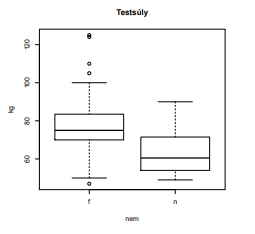
\includegraphics{boxplot}

\section{(172) Irja ra az abrara, hogy melyik tanult eloszlascsalad surusegfuggvenyeit mutatjak be es
egeszítse ki a jelmagyarazatot is.}

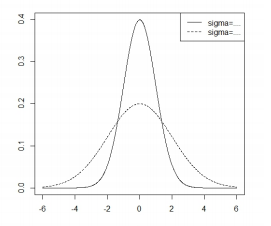
\includegraphics{fuggveny}

 Normalis eloszlasok (0 varhato ertekkel) a folytonos a standard, a szaggatott 2 szorasu
(a surusegfuggveny kepletet egybevetve az abraval leolvashato)


\section{(173) Miert volt erdemes az alabbi modon alkalmazni a hist fuggvenyt? Rajzolja fel a fuggveny eredmenyet! }

\begin{verbatim}
hist(diak[,7],xlab="jegy",ylab="gyakorisag",main="Analízis
jegy",breaks=c(1:6)-1/2)
\end{verbatim}

Azert jo ez az intervallum-beosztas, mert így pontosan kozepre esnek a tenyleges ertekek
es nem keletkeznek "ures" oszlopok, amik a default beallítasnal elofordulhatnak.

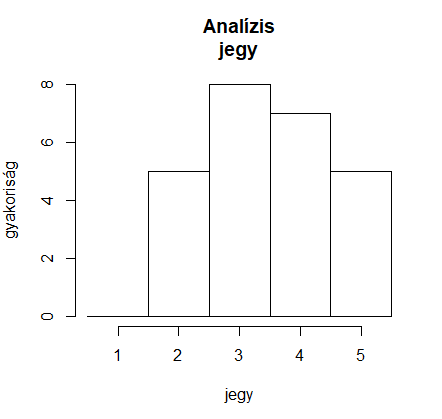
\includegraphics{histogram}

\section{(174)  Mit vizsgaltunk? Mit kaptunk eredmenyul? Mi p.v jelentese?}

\begin{verbatim}
p.v=rep(0,times=365);atlb=p.v;atlk=p.v
for (i in 1:365)
{jan1b<-homb[365*r+i,1];jan1k<-homk[365*r+i,1]
p.v[i]=t.test(jan1b,jan1k,paired=T,alternative="t")\$p.value
atlb[i]=mean(jan1b);atlk[i]=mean(jan1k)}
plot(p.v,type="l")
\end{verbatim}

p.v a p-ertekek vektora az ev napjaira. T-proba

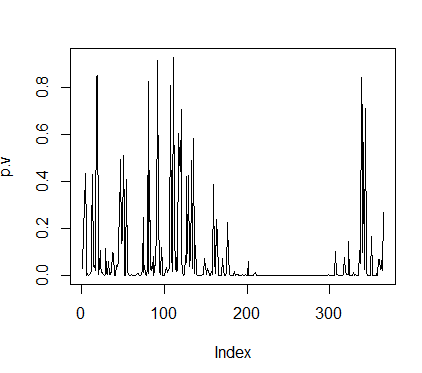
\includegraphics{pv}

\section{(175) Milyen gorbe van az abran? Milyen valoszínusegszamítasi tulajdonsagai vannak?}

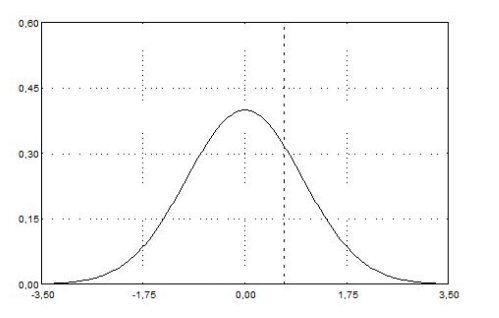
\includegraphics{gorbe}

ez standard normalis eloszlas surusegfuggvenye.


\section{(176) Mit vizsgaltunk? Mit ad meg a p? Egeszítse ki a tablazatot a hianyzo ertekekkel!}

\begin{verbatim}
n<-4;j<-6; q<-c(1:n)/n
h<-c(-Inf,qnorm(q)); mu<-mean(diak[,j])
sig=sd(diak[,j]) ; h<-h*sig+...
nu<-rep(0,times=n)
for (i in 1:n)
nu[i]<- sum((diak[,j]<h[i+1]) & (diak[,j]...h[i]))
np<-sum(nu)*rep(1/n,times=n)
c<-sum((nu-...)^2/np)
p<-1-pchisq(c,n-3)
\end{verbatim}

Linearis modellt illesztettunk a
szeptemberi atlaghumersekletekre a nap sorszamanak fuggvenyeben

A p a p-erteket jeloli.

Kiegeszített valtozat:

\begin{verbatim}
n<-4;j<-6; q<-c(1:n)/n
h<-c(-Inf,qnorm(q)); mu<-mean(diak[,j])
sig=sd(diak[,j]) ; h<-h*sig+mu
nu<-rep(0,times=n)
for (i in 1:n)
nu[i]<- sum((diak[,j]<h[i+1]) & (diak[,j]>=h[i]))
np<-sum(nu)*rep(1/n,times=n)
c<-sum((nu-np)^2/np)
p<-1-pchisq(c,n-3)
\end{verbatim}

N jelentese a mintak szama. $j$ a suly.


\section{(177) Milyen statisztikai fogalmat illusztral az abra? Milyen tulajdonsagai vannak?}

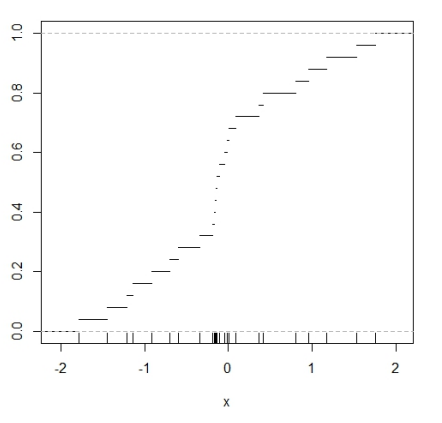
\includegraphics[scale=1.0]{gorbe2}

Ez standard normalis eloszlasu minta tapasztalati eloszlasfuggvenye.

\end{document}